\documentclass{article}
\usepackage[dvipsnames]{xcolor}
\usepackage[paperwidth=9cm, paperheight=6.5cm, margin = 0cm, top=0.25cm]{geometry}

\usepackage{pgf}
\usepackage{tikz}
\usetikzlibrary{arrows,automata}
\usetikzlibrary{positioning}
\tikzstyle{source}  = 
[
	draw,circle,fill=black,thick,inner sep=0mm,minimum size=2mm
]

\tikzstyle{box}  =
[
	draw,rectangle,thick,inner sep=2mm,
	minimum width=8mm, minimum height=8mm
]

\tikzstyle{redbox} = 
[
	draw,rectangle,thick,inner sep=2mm,
	minimum width=8mm, minimum height=8mm,
	fill=red, opacity=0.3, text opacity=1, draw opacity=1
]

\tikzstyle{dredbox} = 
[
	draw,rectangle,thick,inner sep=2mm,
	minimum width=8mm, minimum height=8mm,
	fill=red, opacity=0.5, text opacity=1, draw opacity=1
]


\tikzstyle{bluebox} = 
[
	draw,rectangle,thick,inner sep=2mm,
	minimum width=8mm, minimum height=8mm,
	fill=blue, opacity=0.3, text opacity=1, draw opacity=1
]

\tikzstyle{greenbox} = 
[
	draw,rectangle,thick,inner sep=2mm,
	minimum width=8mm, minimum height=8mm,
	fill=green, opacity=0.3, text opacity=1, draw opacity=1
]

\tikzstyle{lgreenbox} = 
[
	draw,rectangle,thick,inner sep=2mm,
	minimum width=8mm, minimum height=8mm,
	fill=SpringGreen
]

\tikzstyle{dgreenbox} = 
[
	draw,rectangle,thick,inner sep=2mm,
	minimum width=8mm, minimum height=8mm,
	fill=ForestGreen, opacity=0.5, text opacity=1, draw opacity=1
]


\tikzstyle{bluestate}  = 
[
	state, draw=blue, line width=2pt,
	fill=LimeGreen
]

\tikzstyle{redstate}  = 
[
	state, draw=red, line width=2pt,
	fill=LimeGreen
]

\tikzstyle{violetstate}  = 
[
	state, draw=Violet, line width=2pt,
	fill=LimeGreen
]
 

\begin{document}
\begin{center}
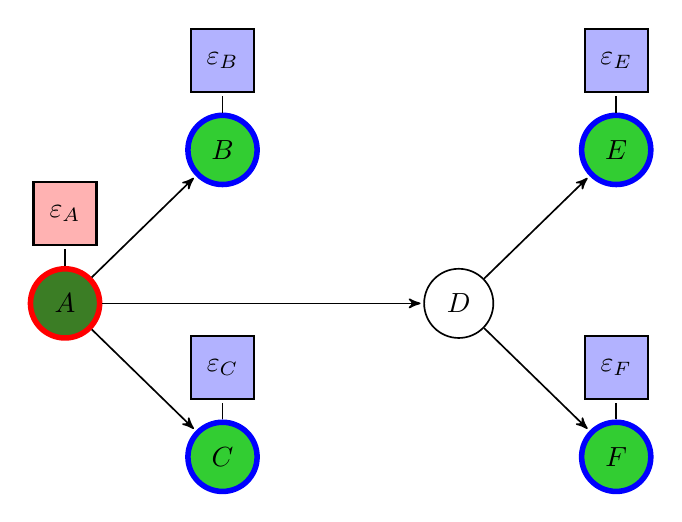
\begin{tikzpicture}[->,>=stealth',shorten >=1pt,auto,node distance=5cm,semithick]
                    
\node[redstate,fill=OliveGreen] (X1) {$A$}; 
\node[bluestate] (X2) [above=1.0cm of X1, xshift=2cm] {$B$};                   
\node[state](X3) [right of=X1] {$D$};
\node[bluestate] (X4) [below=1.0cm of X1, xshift=2cm] {$C$};                   
\node[bluestate] (X5) [right of=X2] {$E$};                   
\node[bluestate] (X6) [right of=X4] {$F$}; 

\node[redbox][above=0.25cm of X1](E1){$\varepsilon_A$};                  
\node[bluebox][above=0.25cm of X2](E2){$\varepsilon_B$};                  
\node[bluebox][above=0.25cm of X4](E4){$\varepsilon_C$};                  
\node[bluebox][above=0.25cm of X5](E5){$\varepsilon_E$};                  
\node[bluebox][above=0.25cm of X6](E6){$\varepsilon_F$};                  

\path
	(X1) edge (X2)
	(X1) edge (X3)
	(X1) edge (X4)
	(X3) edge (X6)
	(X3) edge (X5);

\path
	(X1) edge[-] (E1)
	(X2) edge[-] (E2)
	(X4) edge[-] (E4)
	(X5) edge[-] (E5)
	(X6) edge[-] (E6);

\end{tikzpicture}
\end{center}

\end{document}
